\section{PM-CHECKER}

This section outlines the insights behind \checker's design and implementation.
\Checker models persistent memory, formalizes the correctness and
crash-consistency properties, and provides an API for verifying PM data
structures or PM-Indexes.

\begin{figure}[t]
    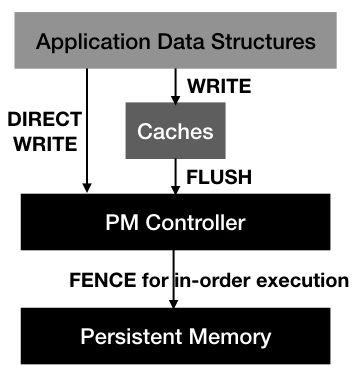
\includegraphics[width=\columnwidth]{figures/nvm-architecture.jpg}
    \caption{\emph{The architecture of Persitent Memory.}}
    \label{fig:architecture}
    \vspace{-0.3in}
\end{figure}


\vheading{Modeling PM.}
PM-CHECKER\footnote{https://github.com/SoujanyaPonnapalli/ASE-396-CourseProject}
models the architecture of persistent memory as shown in the
Figure-\ref{fig:architecture}. The architecture is drawn from the persistent
memory model discussed in ~\cite{blelloch2018parallel}. \Checker aims at
modeling a PM-Index with the following insights:\\
1) \textbf{Capsules}: Code fragments between two fence instructions are termed
Capsules. Capsules are always executed in-order.\\
2) \textbf{Reordering}: Code within every capsule can be reordered by the
PM-Controller. \Checker models capsules using threads and atomic instructions to
synthesize the reordering of PM-Controller.\\
3) \textbf{Idempotency}: \Checker draws parallels between the crash
consistency of PM-indexes with the idempotency of capsules. If the code in a
capsule is idempotent, then it can be shown that the PM-Index is crash
consistent.

\vheading{Correctness and Crash Consistency.}
With the insights of using threads to model instruction reordering, \checker
verifies the correctness of PM-Indexes. Moreover, by maintaining a persistent
queue and a non-volatile queue, \checker can simulate crashes and verify the
idempotency of the code within every capsule.

\vheading{API for Modeling.}
One of the main challenges \checker has to solve, besides modeling persistent
memory and formalizing properties as ltl-formulaes, is to provide the right API
for modeling PM-Indexes.

\vheading{Scalability.}
\Checker is a model checking library that uses SPINs concurrent threads for
simulating instruction reordering and verifying crash-consistency. Both of these
cause the state-space to explode. \Checker has to implement these
functionalities efficiently to scale the verification to concurrent data
structures.

